\documentclass[bsc,letterpaper,12pt]{csthesis}
%\documentclass[letter,12pt,twoside]{csthesis}  para imprimir de lado y lado


\paperwidth = 21.6cm		% Tamaño de la hoja
\paperheight = 27.9cm

%Margenes horizontales
\hoffset = -2.54cm		% Se elimna el offset horizontal
\oddsidemargin = 4cm
\evensidemargin = 2cm
\textwidth = 15.6cm

%Margenes verticales
\voffset = 0.46cm
\topmargin = 0cm
\headheight = 0cm
\headsep = 0cm
\textheight = 21.9cm
\footskip = 1.2cm


\usepackage[spanish]{babel}     % Idioma Capitulos y demas
\usepackage[utf8x]{inputenc}
\usepackage[T1]{fontenc}
\usepackage{lmodern}
\usepackage{cc/CreativeCommons}  %Licencia

\usepackage{listings}
\usepackage{verbatim}
\usepackage{moreverb}
\let\verbatiminput=\verbatimtabinput
\def\verbatimtabsize{8}  % Tabulación en verbatim

% Paquete para el manejo de hipervinculos
\usepackage[colorlinks=true,linkcolor=black,urlcolor=black,citecolor=black, urlcolor=black, filecolor=black]{hyperref}

% Paquete para el manejo de tablas
\usepackage{supertabular}
\usepackage{tabularx}

% Paquete para apendices
\usepackage{appendix}

% Paquetes para simbolos
%\usepackage{mathcomp}
%\usepackage{latexsym}
\usepackage{pifont}
\usepackage{amsfonts}
\usepackage{amssymb}
\usepackage{wasysym}
\usepackage{colortbl}
\usepackage{multicol} 
\usepackage{booktabs}

% Manejo de imagenes PDF y EPS
\newif\ifpdf
\ifx\pdfoutput\undefined
\pdffalse % we are not running PDFLaTeX
\else
\pdfoutput=1 % we are running PDFLaTeX
\pdftrue
\fi

\ifpdf
\usepackage[pdftex]{graphicx}
\else
\usepackage{graphicx}
\fi

\ifpdf
\DeclareGraphicsExtensions{.pdf, .jpg, .tif}
\else
\DeclareGraphicsExtensions{.eps, .jpg}
\fi

% Sangria de comienzo de parrafo
\setlength{\parindent}{0cm}
% Espacio vertical entre dos parrfos
\setlength{\parskip}{0.3cm}

% Definir el nombre de listas
\addto\captionsspanish{%
  \def\prefacename{Prefacio}%
  \def\refname{Referencias}%
  \def\abstractname{RESUMEN}%
  \def\bibname{Bibliograf\'ia}%
  \def\chaptername{Cap\'{\i}tulo}%
  \def\listfigurename{LISTA DE FIGURAS}%
  \def\listtablename{LISTA DE CUADROS}%
  \def\indexname{\'Indice alfab\'etico}%
  \def\figurename{Figura}%
  \def\tablename{Tabla}%
  \def\partname{Parte}%
  \def\enclname{Adjunto}%
  \def\ccname{Copia a}%
  \def\headtoname{A}%
  \def\pagename{P\'agina}%
  \def\seename{v\'ease}%
  \def\alsoname{v\'ease tambi\'en}%
  \def\proofname{Demostraci\'on}%
  \def\glossaryname{GLOSARIO}}%
  \def\appendixname{Ap\'endices}%
  \def\appendixtocname{Ap\'endices}%
  \def\appendixpagename{Ap\'endices}%
  \addto\captionsspanish{\def\contentsname{CONTENIDO}}%


% Inico del documento
\begin{document}
\pagestyle{empty}% Sin número de página
%%% PORTADA


\thispagestyle{empty}

\begin{center}{\centering \large BUSCADOR SEMÁNTICO SAWA}
\end{center}

\vspace{4cm}

\begin{center}{\large OMAR ERNESTO CABRERA ROSERO\\ JIMMY MATEO GUERRERO RESTREPO\\ MAURICIO FERNANDO BENAVIDES BENAVIDES \\ SILVIO RICARDO TIMARÁN PEREIRA}
\end{center}

\vspace{1cm}

\begin{figure}[!h]
\begin{center}

\includegraphics[width=4cm]{pictures/udenar.eps}%logo of your university
\end{center}
\end{figure}

\vspace{1cm}

\begin{center}{\large UNIVERSIDAD DE NARIÑO\\
FACULTAD DE INGENIERÍA\\
PROGRAMA DE INGENIERÍA DE SISTEMAS\\
SAN JUAN DE PASTO\\
2014}
\end{center}

\pagebreak


\newpage
\pagestyle{empty}
\section*{Sobre este trabajo}
\CCbyncsaInfo
\tableofcontents
 
\chapter{Instalación de la aplicación}

Para poder instalar la aplicación debemos instalar PostgreSQL 9.1, Glassfish 3.1.2.2 y la extensión
para postgresql llamada pg\_similarity, la aplicación solo puede ser instalada bajo sistemas
operativos GNU/Linux


Para la instalación de PostgreSQL 9.1 (Para Debian/Linux), en una terminal se ejecuta los siguiente:\\

\lstset{backgroundcolor=\color{white},frame=shadowbox, basicstyle=\small,  breaklines=true, breaklines=true,language=bash}
\begin{lstlisting}
$ su
# apt-get install postgresql postgresql-client pgadmin3
postgresql-server-dev-all postgresql-contrib
\end{lstlisting}

Ahora se borra la contraseña para la cuenta de  administrador de ``postgres'' para ello se ejecuta lo
siguiente en la linea de comandos. \\

\lstset{backgroundcolor=\color{white},frame=shadowbox, basicstyle=\small,  breaklines=true, breaklines=true,language=bash}
\begin{lstlisting}
# su postgres -c psql template1
\end{lstlisting}

\lstset{backgroundcolor=\color{white},frame=shadowbox, basicstyle=\small,  breaklines=true, breaklines=true,language=sql}
\begin{lstlisting}
template1=# ALTER USER postgres WITH PASSWORD `postgres1';
template1=#\q
\end{lstlisting}

Eso altera la contraseña dentro de la base de datos, ahora se tiene que hacer lo mismo para el  
usuario 'postgres' y colocar la misma contraseña que utilizó anteriormente. \\

\lstset{backgroundcolor=\color{white},frame=shadowbox, basicstyle=\small,  breaklines=true, breaklines=true,language=bash}
\begin{lstlisting}
# passwd -d postgres
 #su postgres -c passwd
\end{lstlisting}

Ahora para instalar pg\_similarity primero se descarga desde github de la siguiente manera

\lstset{backgroundcolor=\color{white},frame=shadowbox, basicstyle=\small,  breaklines=true, breaklines=true,language=bash}
\begin{lstlisting}
$ git clone https://github.com/eulerto/pg_similarity.git 
\end{lstlisting}

Luego para que pueda ser usada la extensión se la compila como superusuario de la siguiente manera.

\lstset{backgroundcolor=\color{white},frame=shadowbox, basicstyle=\small,  breaklines=true, breaklines=true,language=bash}
\begin{lstlisting}
# su
# cd pg_similarity
# USE_PGXS=1 make
# USE_PGXS=1 make install
# su postgres
$ createdb sawa
\end{lstlisting}

Luego se crea las funciones y se restaura la copia de la base de datos sawa.sql

\lstset{backgroundcolor=\color{white},frame=shadowbox, basicstyle=\small,  breaklines=true, breaklines=true,language=bash}
\begin{lstlisting}
$ psql sawa
sawa=# create extension pg_similarity;
sawa=# \i sawa.sql
\end{lstlisting}

\textbf{Instalación de Glassfish}

Primero se descarga la versión 3.1.2.2 para GNU/linux desde la página de Oracle\footnote{http://www.oracle.com/technetwork/middleware/glassfish/downloads/ogs-3-1-1-downloads-439803.html}
y se la ejecuta.

\lstset{backgroundcolor=\color{white},frame=shadowbox, basicstyle=\small,  breaklines=true, breaklines=true,language=bash}
\begin{lstlisting}
$ sh ogs-3.1.2.2-unix-ml.sh
\end{lstlisting}

Hay que descargar el driver JDBC de postgresql desde la 
página de PostgreSQL\footnote{http://jdbc.postgresql.org} y copiarlo en 
el directorio glassfish3/glassfish/domains/domain1/lib. Para iniciar el servidor 
se ejecuta lo siguiente


\lstset{backgroundcolor=\color{white},frame=shadowbox, basicstyle=\small,  breaklines=true, breaklines=true,language=bash}
\begin{lstlisting}
$ ./glassfish3/glassfish/bin/startserv
\end{lstlisting}

Con esto ya en en el navegador se inglesa con la dirección http://localhost:8080, y
entramos a la consola de administración, ingresamos usuario y contraseña de haber escrito una
en la instalación de glassfish.

Ir  a ``Resources/JDBC/Connection Pools'' y crear una nueva conexión con los datos que muestra la
Figura~\ref{figura:m1} y luego clic en siguiente.

\begin{figure}[!ht]
\begin{center}
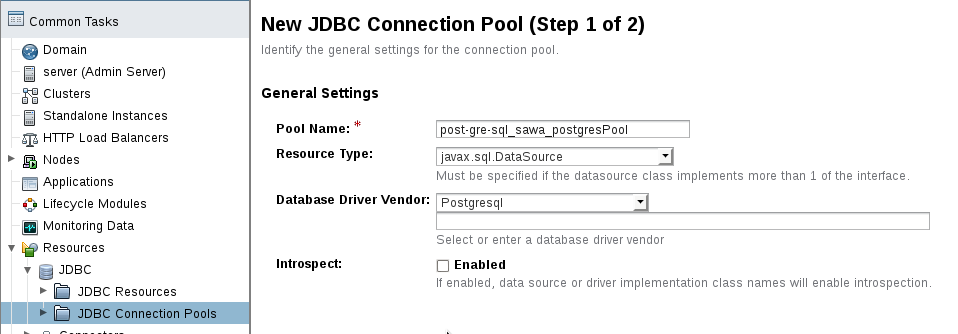
\includegraphics[width=13cm]{pictures/m1.png}
\end{center}
\caption{Crear Nueva conexión} \label{figura:m1}
\end{figure}

Seleccione el origen de datos de nombre de clase org.postgresql.ds.PGConnectionPoolDataSource 
y escribir a las siguientes propiedades adicionales como muestra la Figura~\ref{figura:m2}.

\begin{figure}[!ht]
\begin{center}
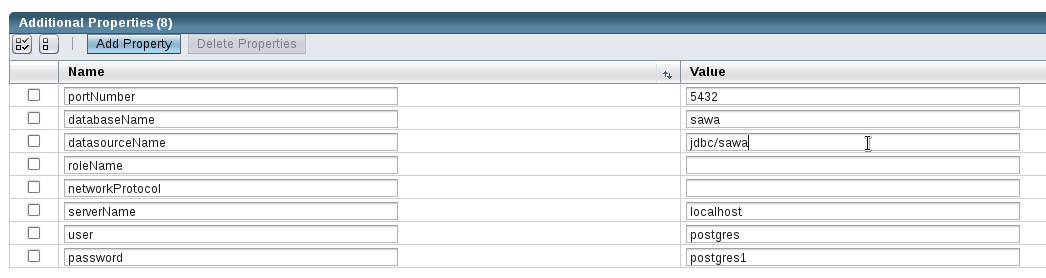
\includegraphics[width=13cm]{pictures/m2.png}
\end{center}
\caption{Propiedades adicionales de conexión} \label{figura:m2}
\end{figure}

Ya con esto guardamos las conexiones y damos clic en finalizar para guardar la conexión.

Luego en ``Resources/JDBC/JDBC Resources'' escribimos en nombre JNDI y escogemos el Pool Name creado 
anteriormente como lo muestra la  Figura~\ref{figura:m3}.

\begin{figure}[!ht]
\begin{center}
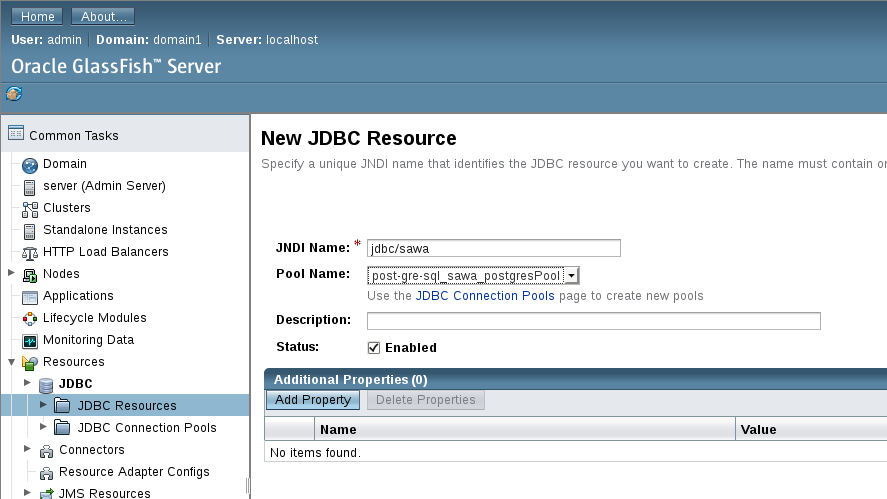
\includegraphics[width=13cm]{pictures/m3.png}
\end{center}
\caption{Recursos JDBC} \label{figura:m3}
\end{figure}

Ya por último en ``Applications'' escogemos en donde tenemos almacenada la aplicación web 
que tiene extensión ``.war'' como muestra la  Figura~\ref{figura:m4}.

\begin{figure}[!ht]
\begin{center}
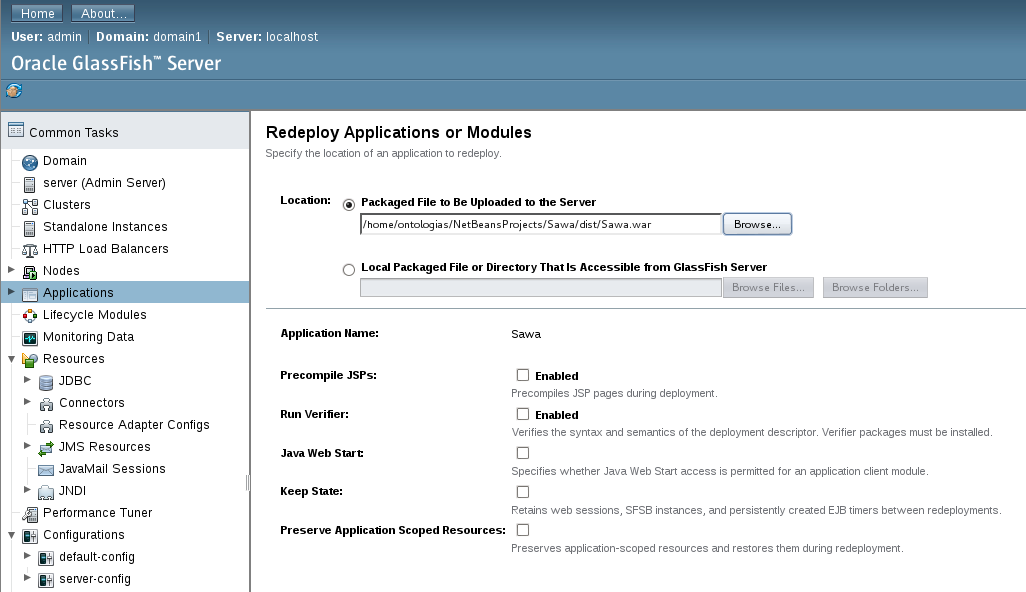
\includegraphics[width=13cm]{pictures/m4.png}
\end{center}
\caption{Subir Aplicación} \label{figura:m4}
\end{figure}

Si todo sale bien nos aparecerá una ventana con la url de la aplicación 
como muestra la Figura~\ref{figura:m5}. y al 
ingresar a la aplicación nos desplegara la ventana de inicio de la aplicación como lo muestra la
Figura~\ref{figura:m6}.

\begin{figure}[!ht]
\begin{center}
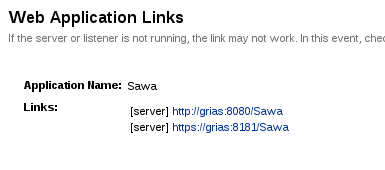
\includegraphics[width=10cm]{pictures/m5.png}
\end{center}
\caption{Url de la Aplicación} \label{figura:m5}
\end{figure}

\begin{figure}[!ht]
\begin{center}
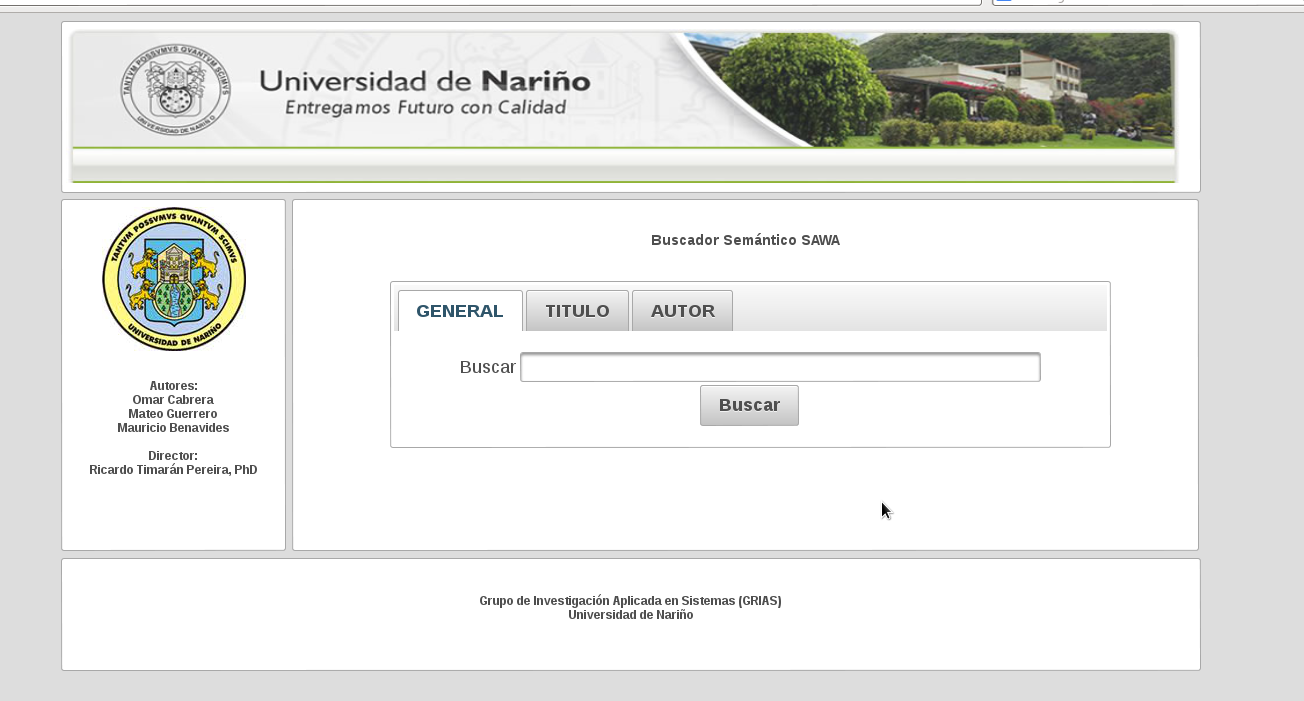
\includegraphics[width=13cm]{pictures/m6.png}
\end{center}
\caption{Aplicación} \label{figura:m6}
\end{figure}

La aplicación esta alojada en \url{http://ingenieria.udenar.edu.co:8080/Sawa/}


 

\end{document}

